\begin{figure}[H]
    \centering
    \caption{Timing of Adoption of \emph{Plan Cuadrante} and Perceived Police Performance}
    \label{fig:balance_doseresponse}
    \begin{subfigure}{0.495\textwidth}
        \centering
        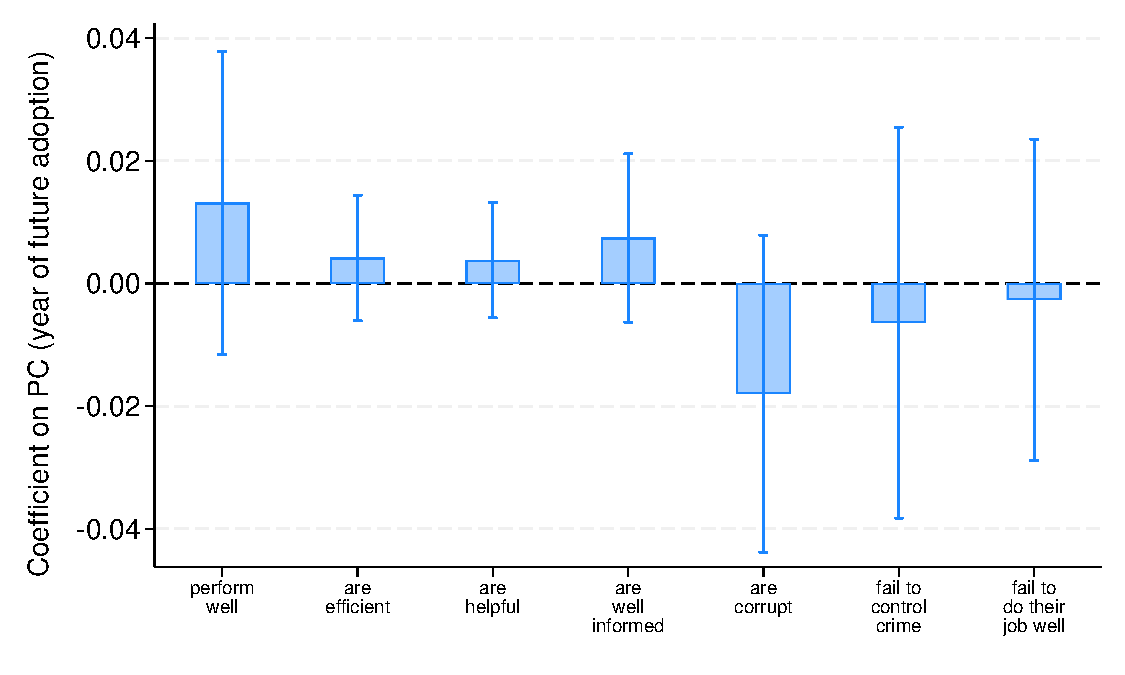
\includegraphics[width=\textwidth]{../manuscript/Graphs/balance_carabperc.pdf}
        \caption{Year of adoption and police performance before adoption}
    \end{subfigure}%
    ~
    \begin{subfigure}{0.495\textwidth}
        \centering
        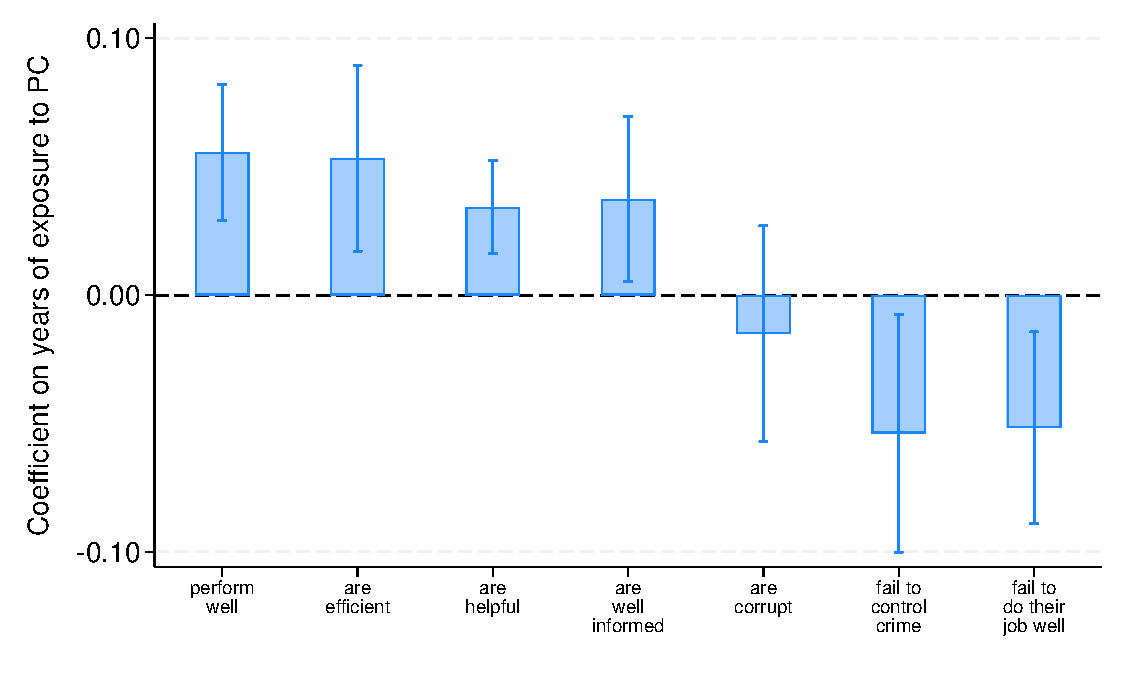
\includegraphics[width=\textwidth]{../manuscript/Graphs/doseresponse_carabperc.pdf}
        \caption{Years exposed to \emph{Plan Cuadrante} (dose response)}
    \end{subfigure}%
    \\[12pt]
    \begin{minipage}{0.99\textwidth}
    Notes: The figure considers seven measures of police performance: the share of respondents who perceive police performance as good, and who perceive the police to be efficient, helpful, well informed, corrupt, failing to control crime, and failing to do their job well. Using the sample of municipalities that adopted \emph{Plan Cuadrante} after 2005, panel (a) examines whether the future timing of adoption of \emph{Plan Cuadrante} is correlated with perceived police performance in 2005, before the introduction of the program. Panel (b) reestimates the same comparison as Figure \ref{fig:figure05}, replacing the binary adoption indicator with the municipality's number of years of exposure to \emph{Plan Cuadrante} as of 2005. In both panels, each bar plots the coefficient from a separate regression of one performance measure. The graphs display the estimated coefficients and 95\% confidence intervals.
    \end{minipage}
\end{figure}
